% !TEX root = ../main.tex

\section{Theory}

% \begin{itemize}
%     \item What is deconvolution and different formulations presented as a review.
%     \item Analysis vs synthesis
%     \begin{itemize}
%         \item TA paper but without the spatial regularization
%         \item PFM paper
%         \item In Gitelman it's an \(\mathbf{H}\) multiplied by a Fourier term.
%     \end{itemize}
%     \item Spikes and block models
% \end{itemize}

\subsection{Notations and definitions}

Matrices of size $N$ rows and $M$ columns are denoted by boldface capital letters, e.g., $\mathbf{X} \in \mathcal{R}^{N\times M}$, whereas column vectors of length $N$ are denoted as boldface lowercase letters, e.g. $\mathbf{x} \in \mathcal{R}^{N}$. Scalars are denoted by lowercase letters, e.g., $k$. Continuous functions are denoted by brackets, e.g., $h(t)$, while discrete functions are denoted by square brackets, e.g., $x[k]$. The euclidean norm of a matrix $\mathbf{X}$ is denoted as $\|\mathbf{X}\|_2$, the $\ell_1$-norm is denoted by $\| \mathbf{X} \|_1$ and the Frobenius norm is denoted by $\| \mathbf{X} \|_F$. %The quadratic distance between two matrices $\mathbf{Y}$ and $\mathbf{X}$ is defined as $\| \mathbf{Y} - \mathbf{X} \|_2^2$.

\subsection{Conventional general linear model analysis}

Conventional general linear model (GLM) analysis puts forward a number of regressors incorporating hypothetical knowledge about the paradigm or behavior. For instance, the timing of epochs for a certain condition can be modeled as an indicator function $p(t)$ (e.g. Dirac functions for event-related designs or box-car functions for block-designs) convolved with the hemodynamic response function (HRF) $h(t)$, and sampled at TR resolution (\citealt{Friston1994AnalysisfunctionalMRI,Friston1998EventRelatedfMRI,Boynton1996LinearSystemsAnalysis,Cohen1997ParametricAnalysisfMRI}):
$$
   p(t) \rightarrow p*h(t) \rightarrow x[k] = p*h(k\cdot\text{TR}).
$$
The vector $\mathbf{x}=[x[k]]_{k=1,\ldots,N}  \in \mathcal{R}^{N}$ then constitutes the regressor modelling the hypothetical response, and several of them can be stacked as columns of the design matrix $\mathbf{X}=[\mathbf{x}_1 \ldots \mathbf{x}_L] \in \mathcal{R}^{N \times L}$, leading to the well-known GLM formulation: 
\begin{equation}
    \label{eq:glm}
    \mathbf{y} = \mathbf{X} \boldsymbol\beta + \mathbf{e},
\end{equation}
where the empirical timecourse $\mathbf{y} \in \mathcal{R}^{N}$ is explained by a linear combination of the regressors in $\mathbf{X}$ weighted by the parameters in $\boldsymbol\beta \in \mathcal{R}^{L}$ and corrupted by additive noise $\mathbf{e}\in \mathcal{R}^{N}$. Under independent and identically distributed Gaussian assumptions of the latter, the maximum likelihood estimate of the parameter weights reverts to the ordinary least-squares estimator; i.e., minimizing the residual sum of squares between the fitted model and measurements. The number of regressors $L$ is typically much less than the number of measurements $N$, and thus the regression problem is over-determined and does no require additional constraints or assumptions.

In the deconvolution approach, no prior knowledge of the hypothetical response is taken into account, and the purpose is to estimate the deconvolved activity-inducing signal $\mathbf{s}$ from the measurements $\mathbf{y}$, which can be formulated as the signal model
\begin{equation}
    \label{eq:synthesis_model}
    \mathbf{y} = \mathbf{Hs} + \mathbf{e},
\end{equation}
where $\mathbf{H} \in \mathcal{N \times N}$ is a Toeplitz matrix that represents the discrete convolution with the HRF, and $\mathbf{s} \in \mathcal{R}^{N}$ is a length-$N$ vector with the unknown activity-inducing signal. Note that the temporal resolution of the activiy-inducing signal and the corresponding Toeplitz matrix is generally assumed to be equal to TR of the acquisition, but it could also be higher if an upsampled estimate is desired. Despite the apparent similarity with the GLM equation, there are two important differences. First, the multiplication with the design matrix of the GLM is an expansion as a weighted linear combination of its columns, while the multiplication with the HRF matrix represents a convolution operator. Second, determining $\mathbf{s}$ is an ill-posed problem given the nature of the HRF. As it can be seen intuitively, the rows of the convolution matrix $\mathbf{H}$ are highly correlated due to large overlap between shifted HRFs (see Figure \ref{fig:sim_and_hrf}C), thus introducing large variability in the estimates of $\mathbf{s}$. Consequently, additional assumptions under the form of regularization terms (or priors) in the estimate are needed to reduce their variance. In the least squares sense, the optimization problem to solve is given as 
\begin{equation}
    \label{eq:regularized_least_squares}
    \hat{\mathbf{s}} = \arg \min_{\mathbf{s}} \frac{1}{2} \| \mathbf{y} - \mathbf{Hs} \|_2^2 + \Omega(\mathbf{s}),
\end{equation}
The first term quantifies data fitness, which can be justified as the log-likelihood term derived from Gaussian noise assumptions, while the second term \(\Omega(\mathbf{s})\) brings in regularization and be interpreted as a prior on the activity-inducing signal. For example, the $\ell_2$-norm of $\mathbf{s}$ is imposed (i.e., $\Omega(\mathbf{s})=\lambda \left\| \mathbf{s}\right\|_2^2$) for ridge regression or Wiener deconvolution, which introduces a trade-off between the data fit term and ``energy'' of the estimates that is controlled by the regularization parameter $\lambda$. %Another well-known regularized terms are related to the elastic net (i.e., $\Omega(\mathbf{x})=\lambda_1\|\mathbf{x}\|_2^2 + \lambda_2\|\mathbf{x}\|_1$) [REF]. 
%%%%%%%%%%%%%%%%%%%%%%%%%%%%%%%%%%%%%%%%%%%%%%%%%%%%%%%%%%%%%%%%%%%%%%%%
% Paradigm Free Mapping
%%%%%%%%%%%%%%%%%%%%%%%%%%%%%%%%%%%%%%%%%%%%%%%%%%%%%%%%%%%%%%%%%%%%%%%%

\subsection{Paradigm free mapping}
 In paradigm free mapping (PFM), the formulation of Eq.~(\ref{eq:regularized_least_squares}) was considered equivalently as fitting the measurements using the atoms of the HRF dictionary (i.e. columns of $\mathbf{H}$) with corresponding weights (entries of $\mathbf{s}$). This model corresponds to a synthesis formulation. In \citealt{Gaudes2013Paradigmfreemapping} a sparsity-pursuing regularization was introduced on $\mathbf{s}$, which in a strict way reverts to choosing \(\Omega(\mathbf{s})=\lambda \| \mathbf{s} \|_0\) as the regularization term and solving the optimization problem (\citealt{Bruckstein2009SparseSolutionsSystems}). However, finding the optimal solution to the problem demands an exhaustive search across all possible combinations of the columns of \(\mathbf{H}\). Hence, a  pragmatic solution is to solve the convex-relaxed optimization problem for the \(l_1\)-norm, commonly known as Basis Pursuit Denoising (\citealt{Chen2001BasisPursuitDenoising}) or equivalently as the least absolute shrinkage and selection operator (LASSO) (\citealt{Tibshirani1996RegressionShrinkageSelection}): 
\begin{equation}
    \label{eq:pfm_spike}
    \hat{\mathbf{s}} = \arg \min_{\mathbf{s}} \frac{1}{2} \| \mathbf{y} - \mathbf{Hs} \|_2^2 + \lambda \| \mathbf{s} \|_1,
\end{equation}
which provides fast convergence to a global solution. Imposing sparsity on the activity-inducing signal implies that it is assumed to be well represented by a reduced subset of very few non-zero coefficients at the fMRI timescale of seconds that trigger brief event-related BOLD responses. Hereinafter, we refer to this assumption as the spike model. 

%%%%%%%%%%%%%%%%%%%%%%%%%%%%%%%%%%%%%%%%%%%%%%%%%%%%%%%%%%%%%%%%%%%%%%%%
% Total Activation
%%%%%%%%%%%%%%%%%%%%%%%%%%%%%%%%%%%%%%%%%%%%%%%%%%%%%%%%%%%%%%%%%%%%%%%%

\subsection{Total activation}
Alternatively, deconvolution can be formulated as a denoising problem where the signal to be recovered is directly fitting the measurements and at the same time satisfying some suitable regularization, which leads to
\begin{equation}
\label{eq:analysis_model}
    \hat{\mathbf{x}} = \arg \min_{\mathbf{x}} \frac{1}{2} \| \mathbf{y} - \mathbf{x} \|_2^2 + \Omega(\mathbf{x}).
\end{equation}
Under this analysis formulation, one powerful regularizer is total variation (TV), which is the $\ell_1$-norm of the derivative, $\Omega(\mathbf{x})=\lambda \|\mathbf{Dx}\|_1$, and favors recovery of piecewise-constant signals (\citealt{Chambolle2004TotalVariation}). Going beyond, the approach of generalized TV introduces an additional differential operator $\mathbf{D_H}$ in the regularizer that can be tailored as the inverse operator of a linear system~(\citealt{Karahanoglu2011SignalProcessingApproach}), that is, $\Omega(\mathbf{x})=\lambda \|\mathbf{D D_H x}\|_1$. In the context of hemodynamic deconvolution, total activation is proposed for which the discrete operator $\mathbf{D_H}$ is derived from the inverse of the continuous-domain linearized Balloon-Windkessel model (\citealt{Buxton1998BalloonModel,Friston2000Nonlinear-Balloon}). \todo{I could exclude this part of Equation 6, and refer to the paper of activelets and TA for more information} Exchanging the poles and zeros of the latter's linear-system characterization leads to a differential operator of the form 
\begin{equation}
    D_H\ = \prod_{i=1}^{M_1} (D-\alpha_i I) (\prod_{j=1}^{M_2} (D - \gamma_j I))^{-1},
\end{equation}
where \(D\) is the derivative operator, \(\alpha_i\) the zeros, and \(\gamma_j\) the poles. The interested reader is referred to (\citealt{Khalidov2011ActiveletsWaveletssparse,Karahanoglu2013TotalactivationfMRI}) for a detailed description. 

Therefore, the solution of the total-activation problem
\begin{equation}
\label{eq:TA}
    \hat{\mathbf{x}} = \arg \min_{\mathbf{x}} \frac{1}{2} \| \mathbf{y} - \mathbf{x} \|_2^2 + \lambda \| \mathbf{D D_H x} \|_1
\end{equation}
will render the activity-related signal $\mathbf{x}$ for which the activity-inducing signal $\mathbf{s}=\mathbf{D_H x}$ and so-called innovation signal $\mathbf{u}=\mathbf{Ds}$ will also be available, as they are required for the regularization. \todo{We might want to include a note that indicates that the TA formulation includes a spatial regularization term that is not considered in the article for the sake of the comparison}We refer to the assumption for the activity-inducing signal as the block model.

\subsection{Unifying both perspectives}

PFM and TA are based on the synthesis- and analysis-based formulation of the deconvolution problem, respectively. In the first case, the recovered deconvolved signal is synthesized to be matched to the measurements, while in the second case, the recovered signal is directly matched to the measurements but needs to satisfy its analysis in terms of deconvolution. This also corresponds to using the forward or backward model of the hemodynamic system, respectively. Both approaches are equivalent\footnote{Without dwelling into technicalities, this equivalence is correct up to the constant, which is in the null space of the derivative operator.} [REF Elad\todo{Would be nice to check a bit closer, this is what I concluded.}]. First, TA can be made equivalent to PFM by removing the derivative operator $\mathbf{D}$ of the regularizer in Eq. (\ref{eq:TA}). It can then be readily verified that replacing in that case $\mathbf{x}=\mathbf{Hs}$ leads to identical equations and thus both assume a spike model \todo{Maybe it is good to indicate that $\mathbf{H}\mathbf{D}_H=\mathbf{I}$}. 

Second, the PFM optimization problem in Eq. (\ref{eq:pfm_spike}) can also be made equivalent to the TA block model in Eq. (\ref{eq:TA}) by considering the modified forward model $\mathbf{y} = \mathbf{H L u} + \mathbf{e}$. Here, the activity-inducing signal $\mathbf{s}$ is rewritten in terms of the innovation signal $\mathbf{u}$ as $\mathbf{s}=\mathbf{Lu}$ where the matrix $\mathbf{L}$ is the first-order integration operator (\citealt{Cherkaoui2019SparsitybasedBlind,Urunuela2020StabilityBasedSparse}) \todo{Do you think it is necessary to define D and L matrices}. This way, PFM can also estimate the innovation signal $\mathbf{u}$ as follows: 
\begin{equation}
    \label{eq:pfm_block}
    \hat{\mathbf{u}} = \arg \min_{\mathbf{u}} \frac{1}{2} \| \mathbf{y} - \mathbf{HLu} \|_2^2 + \lambda \| \mathbf{u} \|_1,
\end{equation}
and becomes equivalent to TA by replacing $\mathbf{u}=\mathbf{D D_H x}$, and thus adopting the block model.

\begin{figure}[t!]
    \begin{center}
        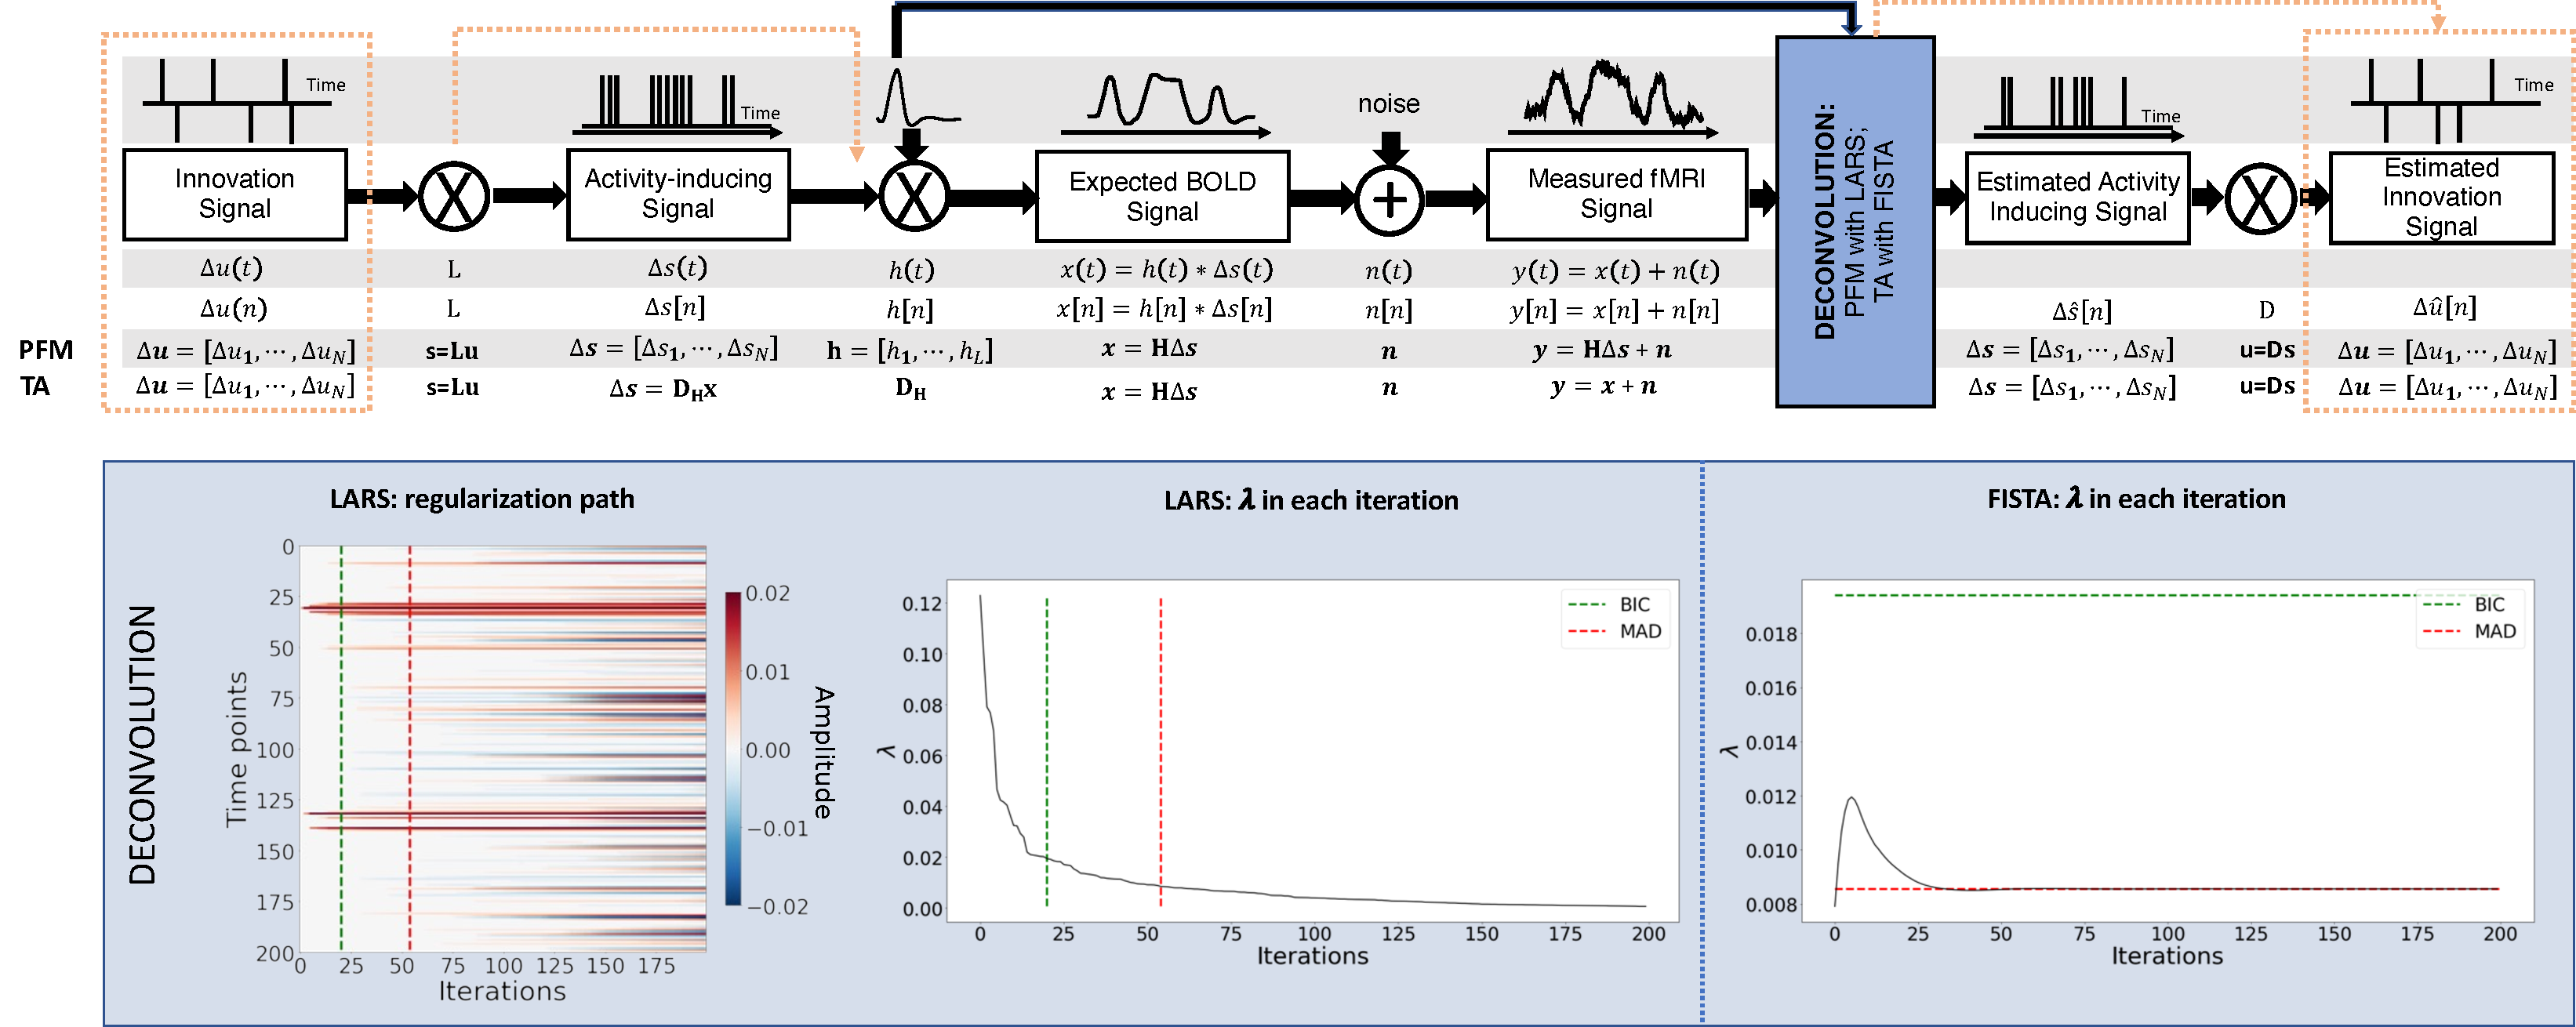
\includegraphics[width=\columnwidth]{figures/flowchart.pdf}
    \end{center}
    \caption{Flowchart detailing the different steps of the fMRI signal and the deconvolution methods described. The orange arrows indicate the flow to estimate the innovation signals. The blue box depicts the two algorithms used in this paper to solve the PFM and TA deconvolution problems.}
\label{fig:flowchart}
\end{figure}

\subsection{Algorithms and parameter selection}
\label{sec:regparam}
Despite their analytical equivalence, both PFM and TA methods are solved with different strategies for the selection of an adequate regularization parameter $\lambda$ and solving the corresponding optimization problem. The PFM implementation available in AFNI employs the least angle regression (LARS) (\citealt{Efron2004Leastangleregression}), whereas the TA implementation uses the fast iterative shrinkage-thresholding algorithm (FISTA) (\citealt{Beck2009FastIterativeShrinkage}). 

On the one hand, LARS is a homotopy approach that computes all the possible solutions to the optimization problem and their corresponding value of $\lambda$, i.e., the regularization path, and the solution according to the Bayesian Information Criterion (BIC) (\citealt{Schwarz1978EstimatingDimensionModel}) is considered appropriate in the case of PFM methods (\citealt{Gaudes2013Paradigmfreemapping,CaballeroGaudes2019deconvolutionalgorithmmulti}). 

Alternatively, the regularization parameter $\lambda$ can also be updated in every iteration of the FISTA so that the residuals of the data fit converge to a previously estimated noise level of the data $\tilde{\sigma}$. This pre-estimated noise level is calculated from the median absolute deviation (MAD) of fine-scale wavelet coefficients (Daubechies, order 3):
\begin{equation}
    \lambda^{n+1} = \frac{N \tilde{\sigma}}{\frac{1}{2} \| \mathbf{y} - \mathbf{x}^n \|_F^2} \lambda^n,
\label{eq:std}
\end{equation}
where $x^n$ is the $n^{th}$ iteration estimate, $\lambda^n$ and $\lambda^{n+1}$ are the $n^{th}$ and $n+1^{th}$ iteration values for the regularization parameter $\lambda$, and $N$ is the number of points in the time-course. %The MAD criterion has been adopted in TA (\citealt{Karahanoglu2013TotalactivationfMRI}), but also in PFM formulations with more extended models (\citealt{Gaudes2012Structuredsparsedeconvolution,Gaudes2011MorphologicalPFM}).

% two techniques, i.e., the regularized least-squares problem with temporal regularization, which corresponds to the generalized total-variation operator in Total Activation. Therefore, we do not study the impact of spatial constraints, as we assume that spatial regularization terms should perform identically on both methods.
